\documentclass{article}

% content/resources/templates/preamble.tex
\usepackage[margin=0.6in]{geometry}
\author{Milav Dabgar}
\usepackage{amsmath,amssymb,amsthm}
\usepackage{booktabs}
\usepackage{multirow}
\usepackage{xcolor}
\usepackage{tcolorbox}
\tcbuselibrary{breakable,skins}
\usepackage[colorlinks=true,linkcolor=blue]{hyperref}
\usepackage{titlesec}
\usepackage{enumitem}
\usepackage{tikz}
\usepackage{pgfplots}
\usepackage{circuitikz}
\usepackage[version=4]{mhchem}
\usepackage{longtable}
\usepackage{array}
\usepackage{float}
\usepackage{caption}
\usepackage{listings}

\lstset{
  basicstyle=\small\ttfamily,
  breaklines=true,
  breakatwhitespace=false,
  postbreak=\mbox{\textcolor{red}{$\hookrightarrow$}\space},
  float=false,
  numbers=left,
  numberstyle=\tiny\color{gray},
  numbersep=10pt,
  xleftmargin=2em,
  keywordstyle=\color{blue},
  commentstyle=\color{green!60!black},
  stringstyle=\color{purple},
  backgroundcolor=\color{gray!5},
  showstringspaces=false,
  tabsize=2,
  captionpos=b,
  keepspaces=true,
  columns=flexible
}

\pgfplotsset{compat=1.18}
\usetikzlibrary{shapes,arrows,positioning,calc,patterns,decorations.pathmorphing,decorations.markings,arrows.meta}

% Color scheme
\definecolor{headcolor}{RGB}{0,102,204}
\definecolor{keycolor}{RGB}{220,20,60}
\definecolor{solutioncolor}{RGB}{34,139,34}
\definecolor{mnemoniccolor}{RGB}{148,0,211}
\definecolor{codecolor}{RGB}{0,0,100}

% Spacing
\setlength{\parskip}{3pt}
\setlist[itemize]{nosep}
\setlist[enumerate]{nosep}

% Title formatting
\titleformat{\section}{\Large\bfseries\color{headcolor}}{\thesection}{1em}{}
\titleformat{\subsection}{\large\bfseries\color{headcolor}}{\thesubsection}{1em}{}

% Pandoc tightlist compatibility
\providecommand{\tightlist}{%
  \setlength{\itemsep}{0pt}\setlength{\parskip}{0pt}}

% Pandoc longtable compatibility
\newcounter{none}
\def\thenone{}


% content/resources/templates/english-boxes.tex
% This file is currently empty - it exists to maintain consistency with the import structure.
% Add custom environments here if needed in the future.


% Custom commands for GTU solutions
% This file defines semantic commands for consistent formatting

% Question command with automatic formatting
\newcommand{\question}[2]{%
  \section*{Question #1}%
  \textbf{#2}%
}

% OR question variant
\newcommand{\questionor}[2]{%
  \section*{Question #1 OR}%
  \textbf{#2}%
}

% Proper table environment with caption
\newenvironment{answertable}[1]{%
  \begin{table}[htbp]
  \centering
  \caption{#1}
}{%
  \end{table}
}

% Proper figure environment for diagrams
\newenvironment{answerdiagram}[1]{%
  \begin{figure}[htbp]
  \centering
  \caption{#1}
}{%
  \end{figure}
}

% Semantic markup for key terms
\newcommand{\keyword}[1]{\textbf{#1}}
\newcommand{\code}[1]{\texttt{#1}}
\newcommand{\classname}[1]{\texttt{#1}}
\newcommand{\methodname}[1]{\texttt{#1}}

% Proper quotation marks
\newcommand{\mnemonic}[1]{``#1''}


\title{Advanced Java Programming (4351603) - Summer 2024 Solution}
\date{May 21, 2024}

\begin{document}
\maketitle

\questionmarks{1(a)}{3}{Explain the difference between AWT and Swing.}

\begin{solutionbox}
\begin{center}
\captionof{table}{AWT vs Swing}
\begin{tabulary}{\linewidth}{|L|L|L|}
\hline
\textbf{Feature} & \textbf{AWT} & \textbf{Swing} \\ \hline
\textbf{Platform} & Platform dependent & Platform independent \\ \hline
\textbf{Components} & Heavy weight & Light weight \\ \hline
\textbf{Look \& Feel} & Native OS look & Pluggable look \& feel \\ \hline
\textbf{Performance} & Faster & Slower than AWT \\ \hline
\end{tabulary}
\end{center}

\textbf{Key Points:}
\begin{itemize}
    \item \keyword{Heavy vs Light}: AWT uses native OS components, Swing uses pure Java.
    \item \keyword{Appearance}: AWT follows OS style, Swing offers consistent look across platforms.
    \item \keyword{Features}: Swing provides more advanced components like JTable, JTree.
\end{itemize}
\end{solutionbox}

\begin{mnemonicbox}
\mnemonic{Swing Provides Lightweight Components}
\end{mnemonicbox}

\questionmarks{1(b)}{4}{Explain Mouse Motion Listener with example.}

\begin{solutionbox}
MouseMotionListener interface handles mouse movement events in Java Swing applications.

\begin{center}
\captionof{table}{Mouse Motion Events}
\begin{tabulary}{\linewidth}{|L|L|}
\hline
\textbf{Method} & \textbf{Purpose} \\ \hline
\textbf{mouseDragged()} & Called when mouse is dragged \\ \hline
\textbf{mouseMoved()} & Called when mouse is moved \\ \hline
\end{tabulary}
\end{center}

\textbf{Code Example:}
\begin{lstlisting}[language=Java]
import javax.swing.*;
import java.awt.event.*;

class MouseMotionExample extends JFrame implements MouseMotionListener {
    JLabel label;
    
    MouseMotionExample() {
        label = new JLabel("Move mouse here");
        add(label);
        addMouseMotionListener(this);
        setSize(400, 300);
        setVisible(true);
    }
    
    public void mouseMoved(MouseEvent e) {
        label.setText("Mouse at: " + e.getX() + ", " + e.getY());
    }
    
    public void mouseDragged(MouseEvent e) {
        label.setText("Dragging at: " + e.getX() + ", " + e.getY());
    }
}
\end{lstlisting}
\end{solutionbox}

\begin{mnemonicbox}
\mnemonic{Mouse Motion Makes Dynamic}
\end{mnemonicbox}

\questionmarks{1(c)}{7}{Develop a program to create checkboxes for different courses belonging to a university such that the course selected would be displayed.}

\begin{solutionbox}
\begin{lstlisting}[language=Java]
import javax.swing.*;
import java.awt.*;
import java.awt.event.*;

public class CourseSelection extends JFrame implements ItemListener {
    JCheckBox java, python, cpp, web;
    JTextArea display;
    
    public CourseSelection() {
        setTitle("University Course Selection");
        setLayout(new FlowLayout());
        
        // Create checkboxes
        java = new JCheckBox("Java Programming");
        python = new JCheckBox("Python Programming");
        cpp = new JCheckBox("C++ Programming");
        web = new JCheckBox("Web Development");
        
        // Add listeners
        java.addItemListener(this);
        python.addItemListener(this);
        cpp.addItemListener(this);
        web.addItemListener(this);
        
        // Display area
        display = new JTextArea(10, 30);
        display.setEditable(false);
        
        // Add components
        add(new JLabel("Select Courses:"));
        add(java); add(python); add(cpp); add(web);
        add(new JScrollPane(display));
        
        setSize(400, 300);
        setDefaultCloseOperation(JFrame.EXIT_ON_CLOSE);
        setVisible(true);
    }
    
    public void itemStateChanged(ItemEvent e) {
        String courses = "Selected Courses:\n";
        if(java.isSelected()) courses += "- Java Programming\n";
        if(python.isSelected()) courses += "- Python Programming\n";
        if(cpp.isSelected()) courses += "- C++ Programming\n";
        if(web.isSelected()) courses += "- Web Development\n";
        display.setText(courses);
    }
    
    public static void main(String[] args) {
        new CourseSelection();
    }
}
\end{lstlisting}

\textbf{Key Features:}
\begin{itemize}
    \item \keyword{ItemListener}: Detects checkbox state changes.
    \item \keyword{Dynamic Display}: Updates selected courses in real-time.
    \item \keyword{Multiple Selection}: Allows selecting multiple courses.
\end{itemize}
\end{solutionbox}

\begin{mnemonicbox}
\mnemonic{Check Items Listen Dynamically}
\end{mnemonicbox}

\questionmarks{1(c OR)}{7}{Develop a program to Implement Traffic signal (Red, Green and Yellow) by using Swing components (Using JFrame, JRadioButton, ItemListener etc.)}

\begin{solutionbox}
\begin{lstlisting}[language=Java]
import javax.swing.*;
import java.awt.*;
import java.awt.event.*;

public class TrafficSignal extends JFrame implements ItemListener {
    JRadioButton red, green, yellow;
    ButtonGroup group;
    JPanel signalPanel;
    
    public TrafficSignal() {
        setTitle("Traffic Signal Simulator");
        setLayout(new BorderLayout());
        
        // Create radio buttons
        red = new JRadioButton("Red");
        green = new JRadioButton("Green"); 
        yellow = new JRadioButton("Yellow");
        
        // Group radio buttons
        group = new ButtonGroup();
        group.add(red); group.add(green); group.add(yellow);
        
        // Add listeners
        red.addItemListener(this);
        green.addItemListener(this);
        yellow.addItemListener(this);
        
        // Signal display panel
        signalPanel = new JPanel() {
            public void paintComponent(Graphics g) {
                super.paintComponent(g);
                g.setColor(Color.BLACK);
                g.fillRect(50, 50, 100, 200);
                
                // Draw circles
                g.setColor(red.isSelected() ? Color.RED : Color.GRAY);
                g.fillOval(65, 65, 70, 70);
                
                g.setColor(yellow.isSelected() ? Color.YELLOW : Color.GRAY);
                g.fillOval(65, 105, 70, 70);
                
                g.setColor(green.isSelected() ? Color.GREEN : Color.GRAY);
                g.fillOval(65, 145, 70, 70);
            }
        };
        
        JPanel controlPanel = new JPanel();
        controlPanel.add(red); controlPanel.add(yellow); controlPanel.add(green);
        
        add(controlPanel, BorderLayout.SOUTH);
        add(signalPanel, BorderLayout.CENTER);
        
        setSize(300, 400);
        setDefaultCloseOperation(JFrame.EXIT_ON_CLOSE);
        setVisible(true);
    }
    
    public void itemStateChanged(ItemEvent e) {
        signalPanel.repaint();
    }
    
    public static void main(String[] args) {
        new TrafficSignal();
    }
}
\end{lstlisting}

\begin{center}
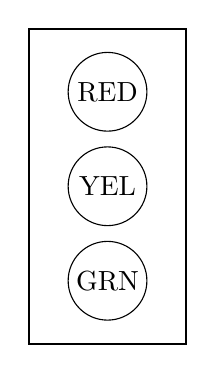
\begin{tikzpicture}
    % Traffic Box
    \draw[thick] (0,0) rectangle (2,4);
    % Circles
    \draw (1,3.2) circle (0.5) node {RED};
    \draw (1,2) circle (0.5) node {YEL};
    \draw (1,0.8) circle (0.5) node {GRN};
\end{tikzpicture}
\captionof{figure}{Traffic Signal Representation}
\end{center}
\end{solutionbox}

\begin{mnemonicbox}
\mnemonic{Radio Buttons Paint Graphics}
\end{mnemonicbox}

\questionmarks{2(a)}{3}{Explain JDBC type-4 driver.}

\begin{solutionbox}
\textbf{JDBC Type-4 Driver (Native Protocol Driver)}

\begin{center}
\captionof{table}{JDBC Type-4 Features}
\begin{tabulary}{\linewidth}{|L|L|}
\hline
\textbf{Feature} & \textbf{Description} \\ \hline
\textbf{Type} & Pure Java driver \\ \hline
\textbf{Communication} & Direct database protocol \\ \hline
\textbf{Platform} & Platform independent \\ \hline
\textbf{Performance} & Highest performance \\ \hline
\end{tabulary}
\end{center}

\textbf{Key Points:}
\begin{itemize}
    \item \keyword{Pure Java}: No native code required.
    \item \keyword{Direct Connection}: Communicates directly with database.
    \item \keyword{Network Protocol}: Uses database's native network protocol.
    \item \keyword{Best Performance}: Fastest among all driver types.
\end{itemize}
\end{solutionbox}

\begin{mnemonicbox}
\mnemonic{Pure Java Direct Protocol}
\end{mnemonicbox}

\questionmarks{2(b)}{4}{Explain Commonly used Methods of Component class.}

\begin{solutionbox}
\begin{center}
\captionof{table}{Component Class Methods}
\begin{tabulary}{\linewidth}{|L|L|}
\hline
\textbf{Method} & \textbf{Purpose} \\ \hline
\textbf{add()} & Adds component to container \\ \hline
\textbf{setSize()} & Sets component dimensions \\ \hline
\textbf{setLayout()} & Sets layout manager \\ \hline
\textbf{setVisible()} & Makes component visible/invisible \\ \hline
\textbf{setBounds()} & Sets position and size \\ \hline
\textbf{getSize()} & Returns component size \\ \hline
\end{tabulary}
\end{center}

\textbf{Key Features:}
\begin{itemize}
    \item \keyword{Layout Management}: Controls component arrangement.
    \item \keyword{Visibility Control}: Shows/hides components.
    \item \keyword{Size Management}: Controls component dimensions.
    \item \keyword{Container Operations}: Manages child components.
\end{itemize}
\end{solutionbox}

\begin{mnemonicbox}
\mnemonic{Add Set Get Visibility}
\end{mnemonicbox}

\questionmarks{2(c)}{7}{Develop a program using JDBC to display student's record (Enroll No, Name, Address, Mobile No and Email-ID) from table 'StuRec'.}

\begin{solutionbox}
\begin{lstlisting}[language=Java]
import java.sql.*;
import javax.swing.*;
import javax.swing.table.DefaultTableModel;

public class StudentRecordDisplay extends JFrame {
    JTable table;
    DefaultTableModel model;
    
    public StudentRecordDisplay() {
        setTitle("Student Records");
        
        // Create table model
        String[] columns = {"Enroll No", "Name", "Address", "Mobile", "Email"};
        model = new DefaultTableModel(columns, 0);
        table = new JTable(model);
        
        // Load data
        loadStudentData();
        
        add(new JScrollPane(table));
        setSize(600, 400);
        setDefaultCloseOperation(JFrame.EXIT_ON_CLOSE);
        setVisible(true);
    }
    
    private void loadStudentData() {
        try {
            // Database connection
            Class.forName("com.mysql.cj.jdbc.Driver");
            Connection con = DriverManager.getConnection(
                "jdbc:mysql://localhost:3306/university", "root", "password");
            
            // Execute query
            Statement stmt = con.createStatement();
            ResultSet rs = stmt.executeQuery("SELECT * FROM StuRec");
            
            // Add data to table
            while(rs.next()) {
                String[] row = {
                    rs.getString("enrollno"),
                    rs.getString("name"),
                    rs.getString("address"),
                    rs.getString("mobile"),
                    rs.getString("email")
                };
                model.addRow(row);
            }
            
            con.close();
        } catch(Exception e) {
            JOptionPane.showMessageDialog(this, "Error: " + e.getMessage());
        }
    }
    
    public static void main(String[] args) {
        new StudentRecordDisplay();
    }
}
\end{lstlisting}

\textbf{Database Table Structure:}
\begin{lstlisting}[language=SQL]
CREATE TABLE StuRec (
    enrollno VARCHAR(20) PRIMARY KEY,
    name VARCHAR(50),
    address VARCHAR(100),
    mobile VARCHAR(15),
    email VARCHAR(50)
);
\end{lstlisting}
\end{solutionbox}

\begin{mnemonicbox}
\mnemonic{Connect Query Display Records}
\end{mnemonicbox}

\questionmarks{2(a OR)}{3}{Write down the advantages and disadvantages of JDBC.}

\begin{solutionbox}
\begin{center}
\captionof{table}{JDBC Advantages and Disadvantages}
\begin{tabulary}{\linewidth}{|L|L|}
\hline
\textbf{Advantages} & \textbf{Disadvantages} \\ \hline
\textbf{Platform Independent} & \textbf{Performance Overhead} \\ \hline
\textbf{Database Independent} & \textbf{Complex for beginners} \\ \hline
\textbf{Standard API} & \textbf{SQL dependency} \\ \hline
\textbf{Supports transactions} & \textbf{Manual resource management} \\ \hline
\end{tabulary}
\end{center}

\textbf{Key Points:}
\begin{itemize}
    \item \keyword{Portability}: Works across different platforms and databases.
    \item \keyword{Standardization}: Uniform API for database operations.
    \item \keyword{Performance}: Additional layer causes overhead.
    \item \keyword{Complexity}: Requires proper resource management.
\end{itemize}
\end{solutionbox}

\begin{mnemonicbox}
\mnemonic{Platform Independent Standard Complex}
\end{mnemonicbox}

\questionmarks{2(b OR)}{4}{Explain Border Layout.}

\begin{solutionbox}
BorderLayout divides container into five regions: North, South, East, West, and Center.

\begin{center}
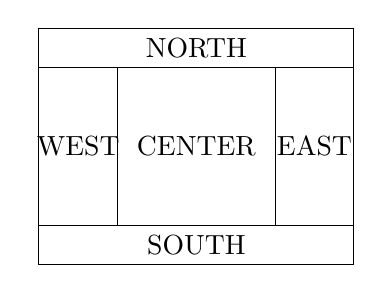
\begin{tikzpicture}
    \draw (0,0) rectangle (4,3);
    \draw (0,2.5) -- (4,2.5);
    \draw (0,0.5) -- (4,0.5);
    \draw (1,0.5) -- (1,2.5);
    \draw (3,0.5) -- (3,2.5);
    
    \node at (2,2.75) {NORTH};
    \node at (2,0.25) {SOUTH};
    \node at (0.5,1.5) {WEST};
    \node at (3.5,1.5) {EAST};
    \node at (2,1.5) {CENTER};
\end{tikzpicture}
\captionof{figure}{Border Layout Regions}
\end{center}

\begin{center}
\captionof{table}{Border Layout Regions}
\begin{tabulary}{\linewidth}{|L|L|L|}
\hline
\textbf{Region} & \textbf{Position} & \textbf{Behavior} \\ \hline
\textbf{NORTH} & Top & Preferred height, full width \\ \hline
\textbf{SOUTH} & Bottom & Preferred height, full width \\ \hline
\textbf{EAST} & Right & Preferred width, full height \\ \hline
\textbf{WEST} & Left & Preferred width, full height \\ \hline
\textbf{CENTER} & Middle & Takes remaining space \\ \hline
\end{tabulary}
\end{center}

\textbf{Code Example:}
\begin{lstlisting}[language=Java]
setLayout(new BorderLayout());
add(new JButton("North"), BorderLayout.NORTH);
add(new JButton("Center"), BorderLayout.CENTER);
\end{lstlisting}
\end{solutionbox}

\begin{mnemonicbox}
\mnemonic{North South East West Center}
\end{mnemonicbox}

\questionmarks{2(c OR)}{7}{Develop an application to store, update, fetch and delete data of Employee (NAME, AGE, SALARY and DEPARTMENT) using Hibernate CRUD operations.}

\begin{solutionbox}
\textbf{Employee Entity Class:}
\begin{lstlisting}[language=Java]
import javax.persistence.*;

@Entity
@Table(name = "employees")
public class Employee {
    @Id
    @GeneratedValue(strategy = GenerationType.IDENTITY)
    private int id;
    
    private String name;
    private int age;
    private double salary;
    private String department;
    
    // Constructors, getters, setters
    public Employee() {}
    
    public Employee(String name, int age, double salary, String dept) {
        this.name = name;
        this.age = age;
        this.salary = salary;
        this.department = dept;
    }
    
    // Getters and Setters
    public int getId() { return id; }
    public void setId(int id) { this.id = id; }
    
    public String getName() { return name; }
    public void setName(String name) { this.name = name; }
    
    // ... other getters/setters
}
\end{lstlisting}

\textbf{CRUD Operations Class:}
\begin{lstlisting}[language=Java]
import org.hibernate.*;
import org.hibernate.cfg.Configuration;

public class EmployeeCRUD {
    private SessionFactory factory;
    
    public EmployeeCRUD() {
        factory = new Configuration()
                    .configure("hibernate.cfg.xml")
                    .addAnnotatedClass(Employee.class)
                    .buildSessionFactory();
    }
    
    // CREATE
    public void saveEmployee(Employee emp) {
        Session session = factory.openSession();
        Transaction tx = session.beginTransaction();
        session.save(emp);
        tx.commit();
        session.close();
    }
    
    // READ
    public Employee getEmployee(int id) {
        Session session = factory.openSession();
        Employee emp = session.get(Employee.class, id);
        session.close();
        return emp;
    }
    
    // UPDATE
    public void updateEmployee(Employee emp) {
        Session session = factory.openSession();
        Transaction tx = session.beginTransaction();
        session.update(emp);
        tx.commit();
        session.close();
    }
    
    // DELETE
    public void deleteEmployee(int id) {
        Session session = factory.openSession();
        Transaction tx = session.beginTransaction();
        Employee emp = session.get(Employee.class, id);
        session.delete(emp);
        tx.commit();
        session.close();
    }
}
\end{lstlisting}
\end{solutionbox}

\begin{mnemonicbox}
\mnemonic{Save Get Update Delete Hibernate}
\end{mnemonicbox}

\questionmarks{3(a)}{3}{Explain Deployment Descriptor.}

\begin{solutionbox}
Deployment Descriptor (web.xml) is configuration file for web applications containing servlet mappings, initialization parameters, and security settings.

\begin{center}
\captionof{table}{Deployment Descriptor Elements}
\begin{tabulary}{\linewidth}{|L|L|}
\hline
\textbf{Element} & \textbf{Purpose} \\ \hline
\textbf{\textless servlet\textgreater} & Defines servlet configuration \\ \hline
\textbf{\textless servlet-mapping\textgreater} & Maps servlet to URL pattern \\ \hline
\textbf{\textless init-param\textgreater} & Sets initialization parameters \\ \hline
\textbf{\textless welcome-file-list\textgreater} & Default files to serve \\ \hline
\end{tabulary}
\end{center}

\textbf{Key Features:}
\begin{itemize}
    \item \keyword{Configuration}: Central configuration for web app.
    \item \keyword{Servlet Mapping}: URL to servlet mapping.
    \item \keyword{Parameters}: Initialization and context parameters.
    \item \keyword{Security}: Authentication and authorization settings.
\end{itemize}
\end{solutionbox}

\begin{mnemonicbox}
\mnemonic{Web XML Configuration Mapping}
\end{mnemonicbox}

\questionmarks{3(b)}{4}{Explain the difference between get and post method in servlet.}

\begin{solutionbox}
\begin{center}
\captionof{table}{GET vs POST Methods}
\begin{tabulary}{\linewidth}{|L|L|L|}
\hline
\textbf{Feature} & \textbf{GET} & \textbf{POST} \\ \hline
\textbf{Data Location} & URL query string & Request body \\ \hline
\textbf{Data Size} & Limited (2048 chars) & Unlimited \\ \hline
\textbf{Security} & Less secure (visible) & More secure \\ \hline
\textbf{Caching} & Can be cached & Not cached \\ \hline
\textbf{Bookmarking} & Can bookmark & Cannot bookmark \\ \hline
\textbf{Purpose} & Retrieve data & Submit/modify data \\ \hline
\end{tabulary}
\end{center}

\textbf{Key Points:}
\begin{itemize}
    \item \keyword{Visibility}: GET data visible in URL, POST hidden.
    \item \keyword{Capacity}: POST can handle large data.
    \item \keyword{Security}: POST better for sensitive data.
    \item \keyword{Usage}: GET for fetching, POST for form submission.
\end{itemize}
\end{solutionbox}

\begin{mnemonicbox}
\mnemonic{GET Visible Limited, POST Hidden Unlimited}
\end{mnemonicbox}

\questionmarks{3(c)}{7}{Develop a simple servlet program which maintains a counter for the number of times it has been accessed since its loading; initialize the counter using deployment descriptor.}

\begin{solutionbox}
\textbf{Servlet Code:}
\begin{lstlisting}[language=Java]
import java.io.*;
import javax.servlet.*;
import javax.servlet.http.*;

public class CounterServlet extends HttpServlet {
    private int counter;
    
    public void init() throws ServletException {
        String initialValue = getInitParameter("initialCount");
        counter = Integer.parseInt(initialValue);
    }
    
    protected void doGet(HttpServletRequest request, 
                        HttpServletResponse response) 
                        throws ServletException, IOException {
        
        response.setContentType("text/html");
        PrintWriter out = response.getWriter();
        
        synchronized(this) {
            counter++;
        }
        
        out.println("<html><body>");
        out.println("<h2>Page Access Counter</h2>");
        out.println("<p>This page has been accessed " + counter + " times</p>");
        out.println("<p><a href='CounterServlet'>Refresh</a></p>");
        out.println("</body></html>");
        
        out.close();
    }
}
\end{lstlisting}

\textbf{web.xml Configuration:}
\begin{lstlisting}[language=XML]
<?xml version="1.0" encoding="UTF-8"?>
<web-app>
    <servlet>
        <servlet-name>CounterServlet</servlet-name>
        <servlet-class>CounterServlet</servlet-class>
        <init-param>
            <param-name>initialCount</param-name>
            <param-value>0</param-value>
        </init-param>
        <load-on-startup>1</load-on-startup>
    </servlet>
    
    <servlet-mapping>
        <servlet-name>CounterServlet</servlet-name>
        <url-pattern>/counter</url-pattern>
    </servlet-mapping>
</web-app>
\end{lstlisting}

\textbf{Key Features:}
\begin{itemize}
    \item \keyword{Thread Safety}: Synchronized counter increment.
    \item \keyword{Initialization}: Counter initialized from web.xml.
    \item \keyword{Persistent}: Counter maintained across requests.
    \item \keyword{Configuration}: Deployment descriptor setup.
\end{itemize}
\end{solutionbox}

\begin{mnemonicbox}
\mnemonic{Initialize Synchronize Count Display}
\end{mnemonicbox}

\questionmarks{3(a OR)}{3}{Explain the life cycle of a servlet.}

\begin{solutionbox}
\begin{center}
\begin{tikzpicture}[node distance=1.5cm, auto]
    \node [gtu state] (Load) {Loading};
    \node [gtu state, right=of Load] (Init) {init()};
    \node [gtu state, right=of Init] (Serv) {service()};
    \node [gtu state, right=of Serv] (Dest) {destroy()};
    
    \path [gtu arrow] (Load) -- (Init);
    \path [gtu arrow] (Init) -- (Serv);
    \path [gtu arrow] (Serv) -- (Dest);
    
    \path [gtu arrow] (Serv) edge [loop above] node {Requests} (Serv);
\end{tikzpicture}
\captionof{figure}{Servlet Life Cycle}
\end{center}

\begin{center}
\captionof{table}{Servlet Life Cycle Methods}
\begin{tabulary}{\linewidth}{|L|L|L|}
\hline
\textbf{Method} & \textbf{Purpose} & \textbf{Called} \\ \hline
\textbf{init()} & Initialize servlet & Once at startup \\ \hline
\textbf{service()} & Handle requests & For each request \\ \hline
\textbf{destroy()} & Cleanup resources & Once at shutdown \\ \hline
\end{tabulary}
\end{center}

\textbf{Key Points:}
\begin{itemize}
    \item \keyword{Initialization}: Called once when servlet loads.
    \item \keyword{Service}: Handles all client requests.
    \item \keyword{Cleanup}: Called before servlet unloads.
    \item \keyword{Container Managed}: Web container controls lifecycle.
\end{itemize}
\end{solutionbox}

\begin{mnemonicbox}
\mnemonic{Initialize Service Destroy}
\end{mnemonicbox}

\questionmarks{3(b OR)}{4}{Explain Servlet Config class with suitable example.}

\begin{solutionbox}
ServletConfig provides servlet-specific configuration information and initialization parameters.

\begin{center}
\captionof{table}{ServletConfig Methods}
\begin{tabulary}{\linewidth}{|L|L|}
\hline
\textbf{Method} & \textbf{Purpose} \\ \hline
\textbf{getInitParameter()} & Gets init parameter value \\ \hline
\textbf{getInitParameterNames()} & Gets all parameter names \\ \hline
\textbf{getServletContext()} & Gets servlet context \\ \hline
\textbf{getServletName()} & Gets servlet name \\ \hline
\end{tabulary}
\end{center}

\textbf{Example:}
\begin{lstlisting}[language=Java]
public class ConfigServlet extends HttpServlet {
    String databaseURL, username;
    
    public void init() throws ServletException {
        ServletConfig config = getServletConfig();
        databaseURL = config.getInitParameter("dbURL");
        username = config.getInitParameter("dbUser");
    }
    
    protected void doGet(HttpServletRequest request, 
                        HttpServletResponse response) 
                        throws ServletException, IOException {
        
        PrintWriter out = response.getWriter();
        out.println("Database URL: " + databaseURL);
        out.println("Username: " + username);
    }
}
\end{lstlisting}

\textbf{web.xml:}
\begin{lstlisting}[language=XML]
<servlet>
    <servlet-name>ConfigServlet</servlet-name>
    <servlet-class>ConfigServlet</servlet-class>
    <init-param>
        <param-name>dbURL</param-name>
        <param-value>jdbc:mysql://localhost:3306/test</param-value>
    </init-param>
    <init-param>
        <param-name>dbUser</param-name>
        <param-value>root</param-value>
    </init-param>
</servlet>
\end{lstlisting}
\end{solutionbox}

\begin{mnemonicbox}
\mnemonic{Config Gets Parameters Context}
\end{mnemonicbox}

\questionmarks{3(c OR)}{7}{Develop a simple program, when user select the subject code, name of the subject will be displayed using servlet and mysql database.}

\begin{solutionbox}
\textbf{HTML Form (index.html):}
\begin{lstlisting}[language=HTML]
<!DOCTYPE html>
<html>
<head>
    <title>Subject Selection</title>
</head>
<body>
    <h2>Select Subject Code</h2>
    <form action="SubjectServlet" method="get">
        <select name="subjectCode">
            <option value="">Select Subject</option>
            <option value="4351603">4351603</option>
            <option value="4351604">4351604</option>
            <option value="4351605">4351605</option>
        </select>
        <input type="submit" value="Get Subject Name">
    </form>
</body>
</html>
\end{lstlisting}

\textbf{Servlet Code:}
\begin{lstlisting}[language=Java]
import java.io.*;
import java.sql.*;
import javax.servlet.*;
import javax.servlet.http.*;

public class SubjectServlet extends HttpServlet {
    
    protected void doGet(HttpServletRequest request, 
                        HttpServletResponse response) 
                        throws ServletException, IOException {
        
        response.setContentType("text/html");
        PrintWriter out = response.getWriter();
        
        String subjectCode = request.getParameter("subjectCode");
        String subjectName = "";
        
        if(subjectCode != null && !subjectCode.equals("")) {
            try {
                Class.forName("com.mysql.cj.jdbc.Driver");
                Connection con = DriverManager.getConnection(
                    "jdbc:mysql://localhost:3306/university", "root", "password");
                
                PreparedStatement ps = con.prepareStatement(
                    "SELECT subject_name FROM subjects WHERE subject_code = ?");
                ps.setString(1, subjectCode);
                
                ResultSet rs = ps.executeQuery();
                if(rs.next()) {
                    subjectName = rs.getString("subject_name");
                }
                
                con.close();
            } catch(Exception e) {
                subjectName = "Error: " + e.getMessage();
            }
        }
        
        out.println("<html><body>");
        out.println("<h2>Subject Information</h2>");
        if(!subjectName.equals("")) {
            out.println("<p>Subject Code: " + subjectCode + "</p>");
            out.println("<p>Subject Name: " + subjectName + "</p>");
        } else {
            out.println("<p>Please select a subject code</p>");
        }
        out.println("<p><a href='index.html'>Back</a></p>");
        out.println("</body></html>");
    }
}
\end{lstlisting}

\textbf{Database Table:}
\begin{lstlisting}[language=SQL]
CREATE TABLE subjects (
    subject_code VARCHAR(10) PRIMARY KEY,
    subject_name VARCHAR(100)
);

INSERT INTO subjects VALUES 
('4351603', 'Advanced Java Programming'),
('4351604', 'Web Technology'),
('4351605', 'Database Management System');
\end{lstlisting}
\end{solutionbox}

\begin{mnemonicbox}
\mnemonic{Select Query Display Subject}
\end{mnemonicbox}

\questionmarks{4(a)}{3}{Explain JSP life cycle.}

\begin{solutionbox}
\begin{center}
\begin{tikzpicture}[node distance=1.2cm, auto]
    \node [gtu state] (Trans) {Translation};
    \node [gtu state, right=of Trans] (Comp) {Compilation};
    \node [gtu state, right=of Comp] (Load) {Loading};
    \node [gtu state, below=of Trans] (Init) {jspInit()};
    \node [gtu state, right=of Init] (Serv) {\_jspService()};
    \node [gtu state, right=of Serv] (Dest) {jspDestroy()};
    
    \path [gtu arrow] (Trans) -- (Comp);
    \path [gtu arrow] (Comp) -- (Load);
    \path [gtu arrow] (Load) -- (Init);
    \path [gtu arrow] (Init) -- (Serv);
    \path [gtu arrow] (Serv) -- (Dest);
    \path [gtu arrow] (Serv) edge [loop above] node {Requests} (Serv);
\end{tikzpicture}
\captionof{figure}{JSP Life Cycle}
\end{center}

\begin{center}
\captionof{table}{JSP Life Cycle Phases}
\begin{tabulary}{\linewidth}{|L|L|}
\hline
\textbf{Phase} & \textbf{Description} \\ \hline
\textbf{Translation} & JSP to Servlet conversion \\ \hline
\textbf{Compilation} & Servlet to bytecode \\ \hline
\textbf{Loading} & Load servlet class \\ \hline
\textbf{Initialization} & jspInit() called \\ \hline
\textbf{Request Processing} & \_jspService() handles requests \\ \hline
\textbf{Destruction} & jspDestroy() cleanup \\ \hline
\end{tabulary}
\end{center}
\end{solutionbox}

\begin{mnemonicbox}
\mnemonic{Translate Compile Load Initialize Service Destroy}
\end{mnemonicbox}

\questionmarks{4(b)}{4}{Compare JSP and Servlet.}

\begin{solutionbox}
\begin{center}
\captionof{table}{JSP vs Servlet Comparison}
\begin{tabulary}{\linewidth}{|L|L|L|}
\hline
\textbf{Feature} & \textbf{JSP} & \textbf{Servlet} \\ \hline
\textbf{Code Type} & HTML with Java code & Pure Java code \\ \hline
\textbf{Development} & Easier for web designers & Better for Java developers \\ \hline
\textbf{Compilation} & Automatic & Manual \\ \hline
\textbf{Modification} & No restart needed & Restart required \\ \hline
\textbf{Performance} & Slower first request & Faster \\ \hline
\textbf{Maintenance} & Easier & More complex \\ \hline
\end{tabulary}
\end{center}

\textbf{Key Points:}
\begin{itemize}
    \item \keyword{Ease of Use}: JSP easier for presentation layer.
    \item \keyword{Performance}: Servlet better for business logic.
    \item \keyword{Flexibility}: JSP better for dynamic content.
    \item \keyword{Control}: Servlet provides more control.
\end{itemize}
\end{solutionbox}

\begin{mnemonicbox}
\mnemonic{JSP Easy HTML, Servlet Pure Java}
\end{mnemonicbox}

\questionmarks{4(c)}{7}{Develop a JSP web application to display student monthly attendance in each subject of current semester via enrolment number.}

\begin{solutionbox}
\textbf{Input Form (attendance.html):}
\begin{lstlisting}[language=HTML]
<!DOCTYPE html>
<html>
<head>
    <title>Student Attendance</title>
</head>
<body>
    <h2>Check Student Attendance</h2>
    <form action="attendanceCheck.jsp" method="post">
        <table>
            <tr>
                <td>Enrollment Number:</td>
                <td><input type="text" name="enrollNo" required></td>
            </tr>
            <tr>
                <td>Month:</td>
                <td>
                    <select name="month" required>
                        <option value="">Select Month</option>
                        <option value="January">January</option>
                        <option value="February">February</option>
                        <option value="March">March</option>
                    </select>
                </td>
            </tr>
            <tr>
                <td colspan="2">
                    <input type="submit" value="Check Attendance">
                </td>
            </tr>
        </table>
    </form>
</body>
</html>
\end{lstlisting}

\textbf{JSP Page (attendanceCheck.jsp):}
\begin{lstlisting}[language=Java]
<%@ page import="java.sql.*" %>
<%@ page contentType="text/html;charset=UTF-8" %>

<html>
<head>
    <title>Attendance Report</title>
    <style>
        table { border-collapse: collapse; width: 100%; }
        th, td { border: 1px solid black; padding: 8px; text-align: center; }
        th { background-color: #f2f2f2; }
    </style>
</head>
<body>
    <h2>Monthly Attendance Report</h2>
    
    <%
        String enrollNo = request.getParameter("enrollNo");
        String month = request.getParameter("month");
        
        if(enrollNo != null && month != null) {
            try {
                Class.forName("com.mysql.cj.jdbc.Driver");
                Connection con = DriverManager.getConnection(
                    "jdbc:mysql://localhost:3306/university", "root", "password");
                
                // Get student info
                PreparedStatement ps1 = con.prepareStatement(
                    "SELECT name FROM students WHERE enroll_no = ?");
                ps1.setString(1, enrollNo);
                ResultSet rs1 = ps1.executeQuery();
                
                String studentName = "";
                if(rs1.next()) {
                    studentName = rs1.getString("name");
                }
                
                out.println("<p><strong>Student:</strong> " + studentName + 
                           " (" + enrollNo + ")</p>");
                out.println("<p><strong>Month:</strong> " + month + "</p>");
                
                // Get attendance data
                PreparedStatement ps2 = con.prepareStatement(
                    "SELECT s.subject_name, a.total_classes, a.attended_classes, " +
                    "ROUND((a.attended_classes/a.total_classes)*100, 2) as percentage " +
                    "FROM attendance a JOIN subjects s ON a.subject_code = s.subject_code " +
                    "WHERE a.enroll_no = ? AND a.month = ?");
                ps2.setString(1, enrollNo);
                ps2.setString(2, month);
                ResultSet rs2 = ps2.executeQuery();
                
                out.println("<table>");
                out.println("<tr><th>Subject</th><th>Total Classes</th>" +
                           "<th>Attended</th><th>Percentage</th><th>Status</th></tr>");
                
                while(rs2.next()) {
                    String subjectName = rs2.getString("subject_name");
                    int totalClasses = rs2.getInt("total_classes");
                    int attendedClasses = rs2.getInt("attended_classes");
                    double percentage = rs2.getDouble("percentage");
                    String status = percentage >= 75 ? "Good" : "Poor";
                    String rowColor = percentage >= 75 ? "lightgreen" : "lightcoral";
                    
                    out.println("<tr style='background-color:" + rowColor + "'>");
                    out.println("<td>" + subjectName + "</td>");
                    out.println("<td>" + totalClasses + "</td>");
                    out.println("<td>" + attendedClasses + "</td>");
                    out.println("<td>" + percentage + "%</td>");
                    out.println("<td>" + status + "</td>");
                    out.println("</tr>");
                }
                
                out.println("</table>");
                con.close();
                
            } catch(Exception e) {
                out.println("<p style='color:red'>Error: " + e.getMessage() + "</p>");
            }
        }
    %>
    
    <br />
    <a href="attendance.html">Check Another Student</a>
</body>
</html>
\end{lstlisting}
\end{solutionbox}

\begin{mnemonicbox}
\mnemonic{JSP Database Query Display Table}
\end{mnemonicbox}

\questionmarks{4(a OR)}{3}{Explain implicit objects in JSP.}

\begin{solutionbox}
\begin{center}
\captionof{table}{JSP Implicit Objects}
\begin{tabulary}{\linewidth}{|L|L|L|}
\hline
\textbf{Object} & \textbf{Type} & \textbf{Purpose} \\ \hline
\textbf{request} & HttpServletRequest & Gets request data \\ \hline
\textbf{response} & HttpServletResponse & Sends response \\ \hline
\textbf{out} & JspWriter & Output to client \\ \hline
\textbf{session} & HttpSession & Session management \\ \hline
\textbf{application} & ServletContext & Application scope \\ \hline
\textbf{config} & ServletConfig & Servlet configuration \\ \hline
\textbf{pageContext} & PageContext & Page scope access \\ \hline
\textbf{page} & Object & Current servlet instance \\ \hline
\textbf{exception} & Throwable & Error page exception \\ \hline
\end{tabulary}
\end{center}

\textbf{Key Features:}
\begin{itemize}
    \item \keyword{Automatic}: Available without declaration.
    \item \keyword{Scope Access}: Different scope levels.
    \item \keyword{Request Handling}: Input/output operations.
    \item \keyword{Session Management}: User session tracking.
\end{itemize}
\end{solutionbox}

\begin{mnemonicbox}
\mnemonic{Request Response Out Session Application}
\end{mnemonicbox}

\questionmarks{4(b OR)}{4}{Explain why JSP is preferred over servlet.}

\begin{solutionbox}
\begin{center}
\captionof{table}{JSP Advantages over Servlet}
\begin{tabulary}{\linewidth}{|L|L|}
\hline
\textbf{Aspect} & \textbf{JSP Advantage} \\ \hline
\textbf{Development} & Easier HTML integration \\ \hline
\textbf{Maintenance} & Separates presentation from logic \\ \hline
\textbf{Compilation} & Automatic compilation \\ \hline
\textbf{Modification} & No server restart needed \\ \hline
\textbf{Design} & Web designer friendly \\ \hline
\textbf{Code Reuse} & Tag libraries and custom tags \\ \hline
\end{tabulary}
\end{center}

\textbf{Key Points:}
\begin{itemize}
    \item \keyword{Separation of Concerns}: Clear separation of presentation and business logic.
    \item \keyword{Rapid Development}: Faster development cycle.
    \item \keyword{Designer Friendly}: Web designers can work with HTML-like syntax.
    \item \keyword{Automatic Features}: Container handles compilation and lifecycle.
\end{itemize}
\end{solutionbox}

\begin{mnemonicbox}
\mnemonic{Easy HTML Automatic Designer Friendly}
\end{mnemonicbox}

\questionmarks{4(c OR)}{7}{Develop a JSP program to display the grade of a student by accepting the marks of five subjects.}

\begin{solutionbox}
\textbf{Input Form (gradeInput.html):}
\begin{lstlisting}[language=HTML]
<!DOCTYPE html>
<html>
<head>
    <title>Student Grade Calculator</title>
</head>
<body>
    <h2 style="text-align: center;">Student Grade Calculator</h2>
    <form action="gradeCalculator.jsp" method="post">
        <table border="1">
            <tr>
                <td>Student Name:</td>
                <td><input type="text" name="studentName" required></td>
            </tr>
            <!-- Subject inputs (1-5) -->
            <tr>
                <td>Subject 1 Marks:</td>
                <td><input type="number" name="marks1" min="0" max="100" required></td>
            </tr>
            <!-- Repeat for marks2 to marks5 -->
            <tr>
                <td colspan="2" style="text-align: center;">
                    <input type="submit" value="Calculate Grade">
                </td>
            </tr>
        </table>
    </form>
</body>
</html>
\end{lstlisting}

\textbf{JSP Grade Calculator (gradeCalculator.jsp):}
\begin{lstlisting}[language=Java]
<%@ page contentType="text/html;charset=UTF-8" %>
<html>
<head>
    <title>Grade Result</title>
</head>
<body>
    <h2 style="text-align: center;">Grade Report</h2>
    
    <%
        String studentName = request.getParameter("studentName");
        
        // Get marks
        int marks1 = Integer.parseInt(request.getParameter("marks1"));
        int marks2 = Integer.parseInt(request.getParameter("marks2"));
        int marks3 = Integer.parseInt(request.getParameter("marks3"));
        int marks4 = Integer.parseInt(request.getParameter("marks4"));
        int marks5 = Integer.parseInt(request.getParameter("marks5"));
        
        // Calculate total and percentage
        int totalMarks = marks1 + marks2 + marks3 + marks4 + marks5;
        double percentage = totalMarks / 5.0;
        
        // Determine grade
        String grade;
        if(percentage >= 90) grade = "A+";
        else if(percentage >= 80) grade = "A";
        else if(percentage >= 70) grade = "B";
        else if(percentage >= 60) grade = "C";
        else if(percentage >= 50) grade = "D";
        else grade = "F";
        
        String result = percentage >= 50 ? "PASS" : "FAIL";
    %>
    
    <table>
        <tr><th colspan="2">Student Information</th></tr>
        <tr><td><strong>Name:</strong></td><td><%= studentName %></td></tr>
        <tr><th colspan="2">Result Summary</th></tr>
        <tr><td><strong>Total Marks:</strong></td><td><%= totalMarks %> / 500</td></tr>
        <tr><td><strong>Percentage:</strong></td><td><%= String.format("%.2f", percentage) %>%</td></tr>
        <tr><td><strong>Grade:</strong></td><td><%= grade %></td></tr>
        <tr><td><strong>Result:</strong></td><td><%= result %></td></tr>
    </table>
</body>
</html>
\end{lstlisting}
\end{solutionbox}

\begin{mnemonicbox}
\mnemonic{Calculate Total Percentage Grade Result}
\end{mnemonicbox}

\questionmarks{5(a)}{3}{Explain Aspect-oriented programming (AOP).}

\begin{solutionbox}
AOP is programming paradigm that separates cross-cutting concerns from business logic using aspects.

\begin{center}
\captionof{table}{AOP Core Concepts}
\begin{tabulary}{\linewidth}{|L|L|}
\hline
\textbf{Concept} & \textbf{Description} \\ \hline
\textbf{Aspect} & Module encapsulating cross-cutting concern \\ \hline
\textbf{Join Point} & Point in program execution \\ \hline
\textbf{Pointcut} & Set of join points \\ \hline
\textbf{Advice} & Action taken at join point \\ \hline
\textbf{Weaving} & Process of applying aspects \\ \hline
\end{tabulary}
\end{center}

\textbf{Key Benefits:}
\begin{itemize}
    \item \keyword{Separation}: Separates business logic from system services.
    \item \keyword{Modularity}: Improves code modularity.
    \item \keyword{Reusability}: Cross-cutting concerns are reusable.
    \item \keyword{Maintenance}: Easier to maintain and modify.
\end{itemize}
\end{solutionbox}

\begin{mnemonicbox}
\mnemonic{Aspect Join Pointcut Advice Weaving}
\end{mnemonicbox}

\questionmarks{5(b)}{4}{List various features of Servlet.}

\begin{solutionbox}
\begin{center}
\captionof{table}{Servlet Features}
\begin{tabulary}{\linewidth}{|L|L|}
\hline
\textbf{Feature} & \textbf{Description} \\ \hline
\textbf{Platform Independent} & Runs on any server supporting Java \\ \hline
\textbf{Server Independent} & Works with different web servers \\ \hline
\textbf{Protocol Independent} & Supports HTTP, HTTPS, FTP \\ \hline
\textbf{Persistent} & Remains in memory between requests \\ \hline
\textbf{Robust} & Strong memory management \\ \hline
\textbf{Secure} & Built-in security features \\ \hline
\textbf{Portable} & Write once, run anywhere \\ \hline
\textbf{Powerful} & Full Java API access \\ \hline
\end{tabulary}
\end{center}

\textbf{Key Points:}
\begin{itemize}
    \item \keyword{Performance}: Better performance than CGI.
    \item \keyword{Memory Management}: Efficient memory usage.
    \item \keyword{Multithreading}: Handles multiple requests simultaneously.
    \item \keyword{Extensible}: Can be extended for specific protocols.
\end{itemize}
\end{solutionbox}

\begin{mnemonicbox}
\mnemonic{Platform Server Protocol Persistent Robust}
\end{mnemonicbox}

\questionmarks{5(c)}{7}{Explain Model layer, View layer and Controller layer in details.}

\begin{solutionbox}
\begin{center}
\begin{tikzpicture}[node distance=2cm, auto]
    \node [gtu block] (User) {User};
    \node [gtu block, below right=of User] (View) {View};
    \node [gtu block, right=of View] (Cont) {Controller};
    \node [gtu block, above=of Cont] (Model) {Model};
    
    \path [gtu arrow] (User) -- (Cont);
    \path [gtu arrow] (Cont) -- (Model);
    \path [gtu arrow, <->] (Model) -- (View);
    \path [gtu arrow] (View) -- (User);
\end{tikzpicture}
\captionof{figure}{MVC Architecture}
\end{center}

\begin{center}
\captionof{table}{MVC Layer Details}
\begin{tabulary}{\linewidth}{|L|L|L|L|}
\hline
\textbf{Layer} & \textbf{Responsibility} & \textbf{Components} & \textbf{Purpose} \\ \hline
\textbf{Model} & Data and business logic & Entities, DAOs, Services & Data management \\ \hline
\textbf{View} & Presentation layer & JSP, HTML, CSS & User interface \\ \hline
\textbf{Controller} & Request handling & Servlets, Actions & Flow control \\ \hline
\end{tabulary}
\end{center}

\textbf{Layer Details:}
\begin{itemize}
    \item \textbf{Model}: Handles database operations, business logic, validation, and entity classes.
    \item \textbf{View}: Handles presentation, display logic, user interaction, and responsive design.
    \item \textbf{Controller}: Handles requests, flow control, model coordination, and response generation.
\end{itemize}

\textbf{Benefits of MVC:}
\begin{itemize}
    \item \keyword{Separation of Concerns}: Clear responsibility division.
    \item \keyword{Maintainability}: Easier to maintain and modify.
    \item \keyword{Testability}: Each layer can be tested independently.
    \item \keyword{Scalability}: Supports large application development.
\end{itemize}
\end{solutionbox}

\begin{mnemonicbox}
\mnemonic{Model Data View Present Controller Handle}
\end{mnemonicbox}

\questionmarks{5(a OR)}{3}{Explain Features in Spring Boot.}

\begin{solutionbox}
\begin{center}
\captionof{table}{Spring Boot Features}
\begin{tabulary}{\linewidth}{|L|L|}
\hline
\textbf{Feature} & \textbf{Description} \\ \hline
\textbf{Auto Configuration} & Automatic configuration based on dependencies \\ \hline
\textbf{Starter Dependencies} & Curated set of dependencies \\ \hline
\textbf{Embedded Servers} & Built-in Tomcat, Jetty servers \\ \hline
\textbf{Production Ready} & Health checks, metrics, monitoring \\ \hline
\textbf{No XML Configuration} & Annotation-based configuration \\ \hline
\textbf{Developer Tools} & Hot reloading, automatic restart \\ \hline
\end{tabulary}
\end{center}

\textbf{Key Benefits:}
\begin{itemize}
    \item \keyword{Rapid Development}: Quick project setup and development.
    \item \keyword{Convention over Configuration}: Sensible defaults.
    \item \keyword{Microservices Ready}: Easy microservices development.
\end{itemize}
\end{solutionbox}

\begin{mnemonicbox}
\mnemonic{Auto Starter Embedded Production Annotation Developer}
\end{mnemonicbox}

\questionmarks{5(b OR)}{4}{Write Short note on JSP scripting elements.}

\begin{solutionbox}
\begin{center}
\captionof{table}{JSP Scripting Elements}
\begin{tabulary}{\linewidth}{|L|L|L|}
\hline
\textbf{Element} & \textbf{Syntax} & \textbf{Purpose} \\ \hline
\textbf{Scriptlet} & \code{<\% \%>} & Java code execution \\ \hline
\textbf{Expression} & \code{<\%= \%>} & Output value \\ \hline
\textbf{Declaration} & \code{<\%! \%>} & Variable/method declaration \\ \hline
\textbf{Directive} & \code{<\%@ \%>} & Page configuration \\ \hline
\textbf{Comment} & \code{<\%-- --\%>} & JSP comments \\ \hline
\end{tabulary}
\end{center}

\textbf{Example:}
\begin{lstlisting}[language=Java]
<%-- JSP Comment --%>
<%@ page contentType="text/html" %>

<%! 
    private int counter = 0;
%>

<html>
<body>
    <% 
        String name = "Student";
        counter++;
    %>
    
    <h1><%= "Welcome " + name %></h1>
    <p>Page visited <%= counter %> times</p>
</body>
</html>
\end{lstlisting}
\end{solutionbox}

\begin{mnemonicbox}
\mnemonic{Script Express Declare Direct Comment}
\end{mnemonicbox}

\questionmarks{5(c OR)}{7}{Explain Dependency injection (DI) and Plain Old Java Object (POJO) in details.}

\begin{solutionbox}
\textbf{Dependency Injection (DI):}
Dependency Injection is design pattern where objects receive their dependencies from external source rather than creating them internally.

\begin{center}
\captionof{table}{DI Types}
\begin{tabulary}{\linewidth}{|L|L|L|}
\hline
\textbf{Type} & \textbf{Description} & \textbf{Example} \\ \hline
\textbf{Constructor} & Dependencies via constructor & \code{public Service(Repo r)} \\ \hline
\textbf{Setter} & Dependencies via setter methods & \code{setRepo(Repo r)} \\ \hline
\textbf{Field} & Direct field injection & \code{@Autowired Repo r} \\ \hline
\end{tabulary}
\end{center}

\textbf{Plain Old Java Object (POJO):}
POJO is simple Java object that doesn't inherit from any specific framework classes or implement specific interfaces.

\textbf{POJO Characteristics:}
\begin{itemize}
    \item \keyword{No inheritance}: Doesn't extend framework classes.
    \item \keyword{No interfaces}: Doesn't implement framework interfaces.
    \item \keyword{No annotations}: Can work without framework annotations.
    \item \keyword{Simple}: Contains only business logic and data.
\end{itemize}

\textbf{Example:}
\begin{lstlisting}[language=Java]
// POJO Entity
public class Student {
    private String name;
    // constructors, getters, setters
}

// Service with DI
@Service
public class StudentService {
    @Autowired
    private StudentRepository repository;
    
    public void save(Student s) {
        repository.save(s);
    }
}
\end{lstlisting}

\textbf{Benefits:}
\begin{itemize}
    \item \keyword{DI}: Loose coupling, Testability, Flexibility.
    \item \keyword{POJO}: Simplicity, Testability, Portability, Lightweight.
\end{itemize}
\end{solutionbox}

\begin{mnemonicbox}
\mnemonic{DI Injects Dependencies, POJO Plain Objects}
\end{mnemonicbox}

\end{document}
